\section{Implementation and Performance Evaluation}
\label{sec:eval}

\subsection{Environment and implementation}

We use UavNetSim-v1~\cite{zhou2025uavnetsim}, a discrete-event simulator written in Python on SimPy, pinned at
tag v1.0.1~\cite{zhou2026repo}, with Python 3.12. LEAP-GR is a new module in \texttt{routing/leap/} that
implements the platform's routing interface (\texttt{next\_hop\_selection}, \texttt{packet\_reception},
\texttt{penalize}). Our changes to the simulator are small and listed in the repository: configuration
parameters for speed, traffic rate and protocol, a protocol registry, the observe-only hooks of
\cref{sec:attribution}, and energy depletion disabled. Without the last change, every UAV runs out of
battery and stops after about 14--19\,s of a 30\,s run, earlier at low speed, which would distort the speed
sweep. With identical seeds, the hooks leave all upstream metrics bit-identical (golden test).

\subsection{Scenarios and statistics}

\Cref{tab:params} lists the parameters. We vary one factor at a time around a reference point ($N=30$,
$\bar v=10$\,m/s, $\lambda=1$ packet/s per UAV): $N\in\{10,\dots,50\}$, $\bar v\in\{5,10,15,20\}$\,m/s and
$\lambda\in\{0.5,1,2,5\}$, which gives 11 configurations. Every UAV generates traffic, so in the $N$ sweep the
offered load $N\lambda$ grows with density; we read that sweep together with the $\lambda$ sweep. Each
configuration runs with seeds 1--3. A seed fixes trajectories and traffic for all protocols, so differences
are \emph{paired}: we report means with 95\,\% Student-$t$ confidence intervals (CIs) and test differences with
a paired $t$-test. We call a difference significant only if its paired CI excludes zero. The threshold
$\tauth$ was chosen on separate seeds (100--102), never on the test seeds. The same seed and code version
reproduce a run exactly: four runs computed on two different machines gave identical results.

\begin{table}[t]
\centering
\caption{Simulation parameters (platform defaults unless stated).}
\label{tab:params}
\footnotesize
\begin{tabular}{@{}p{2.6cm}p{5.6cm}@{}}
\toprule
Parameter & Value \\
\midrule
Area & $600\times600\times100$\,m \\
UAVs $N$ & 10, 20, \textbf{30}, 40, 50 \\
Mobility & 3-D Gauss--Markov, $\alpha=0.85$, mean speed 5, \textbf{10}, 15, 20\,m/s \\
Traffic & Poisson, $\lambda=0.5$, \textbf{1}, 2, 5 packets/s per UAV, random destination \\
Payload & 1024\,B \\
PHY & free space, $P_t=0.1$\,W, $f_c=2.4$\,GHz, SINR $\ge6$\,dB, $\Rmax=249.3$\,m \\
MAC & CSMA/CA with ACK, 2\,Mbit/s, $\le5$ attempts per hop \\
Queue / packet lifetime & 200 packets / 10\,s \\
Hello period / neighbour lifetime & 0.5\,s / 2\,s (Greedy and LEAP-GR) \\
LEAP-GR & $\kappa=0.9$, $\tauth$ from \cref{sec:tau}, +128\,bit per hello \\
Run & 30\,s, traffic in $[2, 27]$\,s, energy depletion off \\
Seeds & 1--3 (test), 100--102 (tuning of $\tauth$) \\
\bottomrule
\end{tabular}
\end{table}

\subsection{Diagnosis of the existing protocols}
\label{sec:diag}

\begin{figure*}[t]
\centering
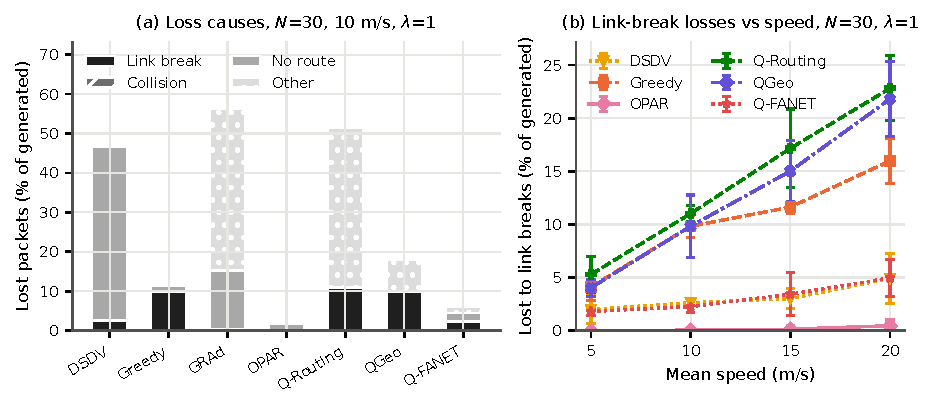
\includegraphics[width=\textwidth]{fig2_loss_causes}
\caption{(a) Final cause of lost packets, as a percentage of generated packets, at the reference point
($N=30$, 10\,m/s, $\lambda=1$, mean of 3 seeds). (b) Packets lost to link breaks versus mean speed for the
unicast protocols (GRAd broadcasts and has no link-break losses by construction). Error bars: 95\,\% CI.}
\label{fig:losses}
\end{figure*}

\Cref{fig:losses}a breaks down the losses of the seven protocols at the reference point. Two results stand
out. First, \emph{collisions are almost never the final cause of a loss}: at most 0.09\,\% of generated packets
for the unicast protocols (0.42\,\% for GRAd, which has no retransmissions), against 9.8\,\% lost to link breaks for Greedy. A collision costs one MAC attempt, and the
next attempt usually succeeds, so the five-attempt budget absorbs collisions. A link break does not go away
between attempts: the MAC resends the same frame to a neighbour that has left, five times, and drops it. Of
the losses that are either link breaks or collisions, link breaks account for 99--100\,\% for every unicast
protocol. Even at $\lambda=5$, where the channel saturates, collision losses stay below 0.01\,\% for Greedy;
congestion then shows up as packets that expire in queues (8.2\,\% of Greedy's packets) and as packets
without a route, not as collisions.

Second, the protocols fail in different ways. Link breaks cause 83\,\% of Greedy's losses. DSDV loses
44\,\% of its packets for lack of a route: its tables lag behind the topology. GRAd loses packets to queue
overflow (24.5\,\%) and to missing routes (14.7\,\%), because every relay rebroadcasts. Q-Routing's delivered packets
travel 6.6 hops on average against 1.8 for Greedy, and 40\,\% of its packets expire: its learned estimates
send packets on long detours. OPAR, which reads the true positions and velocities of all UAVs, delivers 97.7\,\%
and loses almost nothing to link breaks; it shows what prediction can achieve with global knowledge.

\Cref{fig:losses}b shows that link-break losses grow with speed for every distributed unicast protocol:
from 4.1\,\% of generated packets at 5\,m/s to 16.0\,\% at 20\,m/s for Greedy, and from 5.3\,\% to 22.8\,\%
for Q-Routing. At 20\,m/s link breaks cause all of Greedy's losses. Faster UAVs cross the 249\,m range sooner,
while the 2\,s neighbour lifetime keeps departed neighbours in the table.

\begin{figure}[t]
\centering
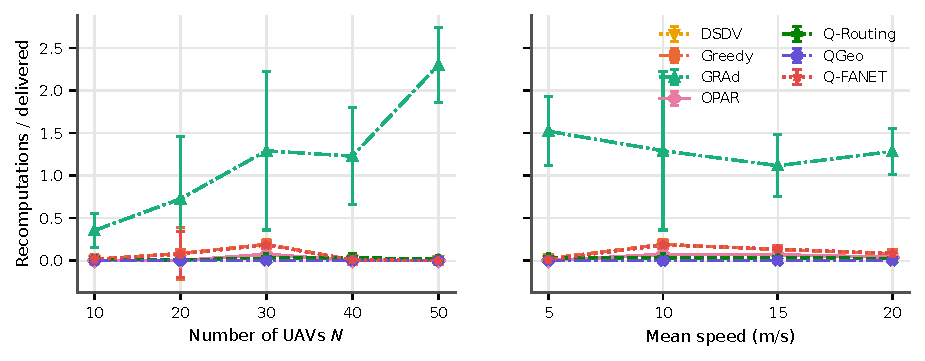
\includegraphics[width=\columnwidth]{fig3_recomputations}
\caption{Route recomputations per delivered packet versus $N$ and mean speed (3 seeds, 95\,\% CI).}
\label{fig:rr}
\end{figure}

\Cref{fig:rr} shows route recomputations per delivered packet. GRAd recomputes most, 1.3 per delivered
packet at the reference point, mostly route-request broadcasts (0.84 per delivered packet) plus
waiting-list retries (0.38).
Greedy recomputes 0.19 times per delivered packet, all of them waiting-list retries. Greedy's MAC retries
are not recomputations: they go to the same neighbour. That is the gap LEAP-GR targets: Greedy keeps no
alternative when a link fails, and its retries are spent on a neighbour that has already left.

\subsection{Choice of the threshold}
\label{sec:tau}

\pending{Fig.~7 (re-run of Exp C on tuning seeds 100--102, $N=30$, 20\,m/s, $\lambda=1$): PDR, proactive
switches and shadow-mode precision/recall versus $\tauth$; the frozen value and why PDR falls for large
$\tauth$. Shadow-mode facts (unaffected by the fix): recall 680/680 at every window; precision 0.40 to 0.56
from 0.25 to 4\,s; median lead time about 4.5\,ms, i.e.\ most warnings concern neighbours that have already
left.}

\subsection{Comparison with Greedy and GRAd}
\label{sec:comparison}

\pending{Fig.~4 (PDR over the three sweeps: Greedy, GRAd, reactive control, LEAP-GR) and Fig.~5 (delay and
control traffic). Text: figure, what it shows, why, takeaway. Paired table from \texttt{table\_paired.csv}.}

\subsection{Isolating the gain of prediction}
\label{sec:ablation}

\pending{Fig.~6 and Table~III: paired differences A1$-$A0, A2$-$A0, R$-$A0, A2$-$R per configuration;
where prediction beats reacting and where it does not, and the mechanism (stale-neighbour filtering versus
anticipation).}

\subsection{Cross-layer weighting}
\label{sec:xl}

\pending{Exp D: LEAP-GR vs LEAP-GR with cross-layer weighting on the speed sweep and at $\lambda=5$; with few
ACK timeouts at $\lambda=1$ the weights stay near zero and the ranking does not change.}

\subsection{Threats to validity}

The channel is free space without fading, which makes link breaks exact and predictable from distance; a
fading channel would blur the range edge and lower prediction precision. Mobility is Gauss--Markov only.
Like Greedy, LEAP-GR assumes that the source knows the destination's position. OPAR uses global knowledge
on this platform. GRAd forwards by broadcast without ACKs, as implemented upstream, so its MAC behaviour
differs by design even though the MAC protocol and parameters are the same. Runs last 30\,s with three seeds
per configuration; paired statistics compensate in part. Energy depletion is disabled. In the $N$ sweep,
density and offered load vary together.
